% A workaround to allow relative paths in included subfiles
% that are to be compiled separately
% See https://tex.stackexchange.com/questions/153312/subfiles-inside-a-subfile-using-relative-paths
\providecommand{\main}{..}
\documentclass[\main/thesis.tex]{subfiles}

\begin{document}

\chapter{Results}

We collected our results by using Weights \& Biases framework. We created several
graphs from the raw data to showcase how the two models perform for the various GLUE tasks. 


\section{CoLA Results}\label{sec:cola_results}

We will start with the CoLA results where we saw the most different between the two models. 

\begin{figure}
    \centering
    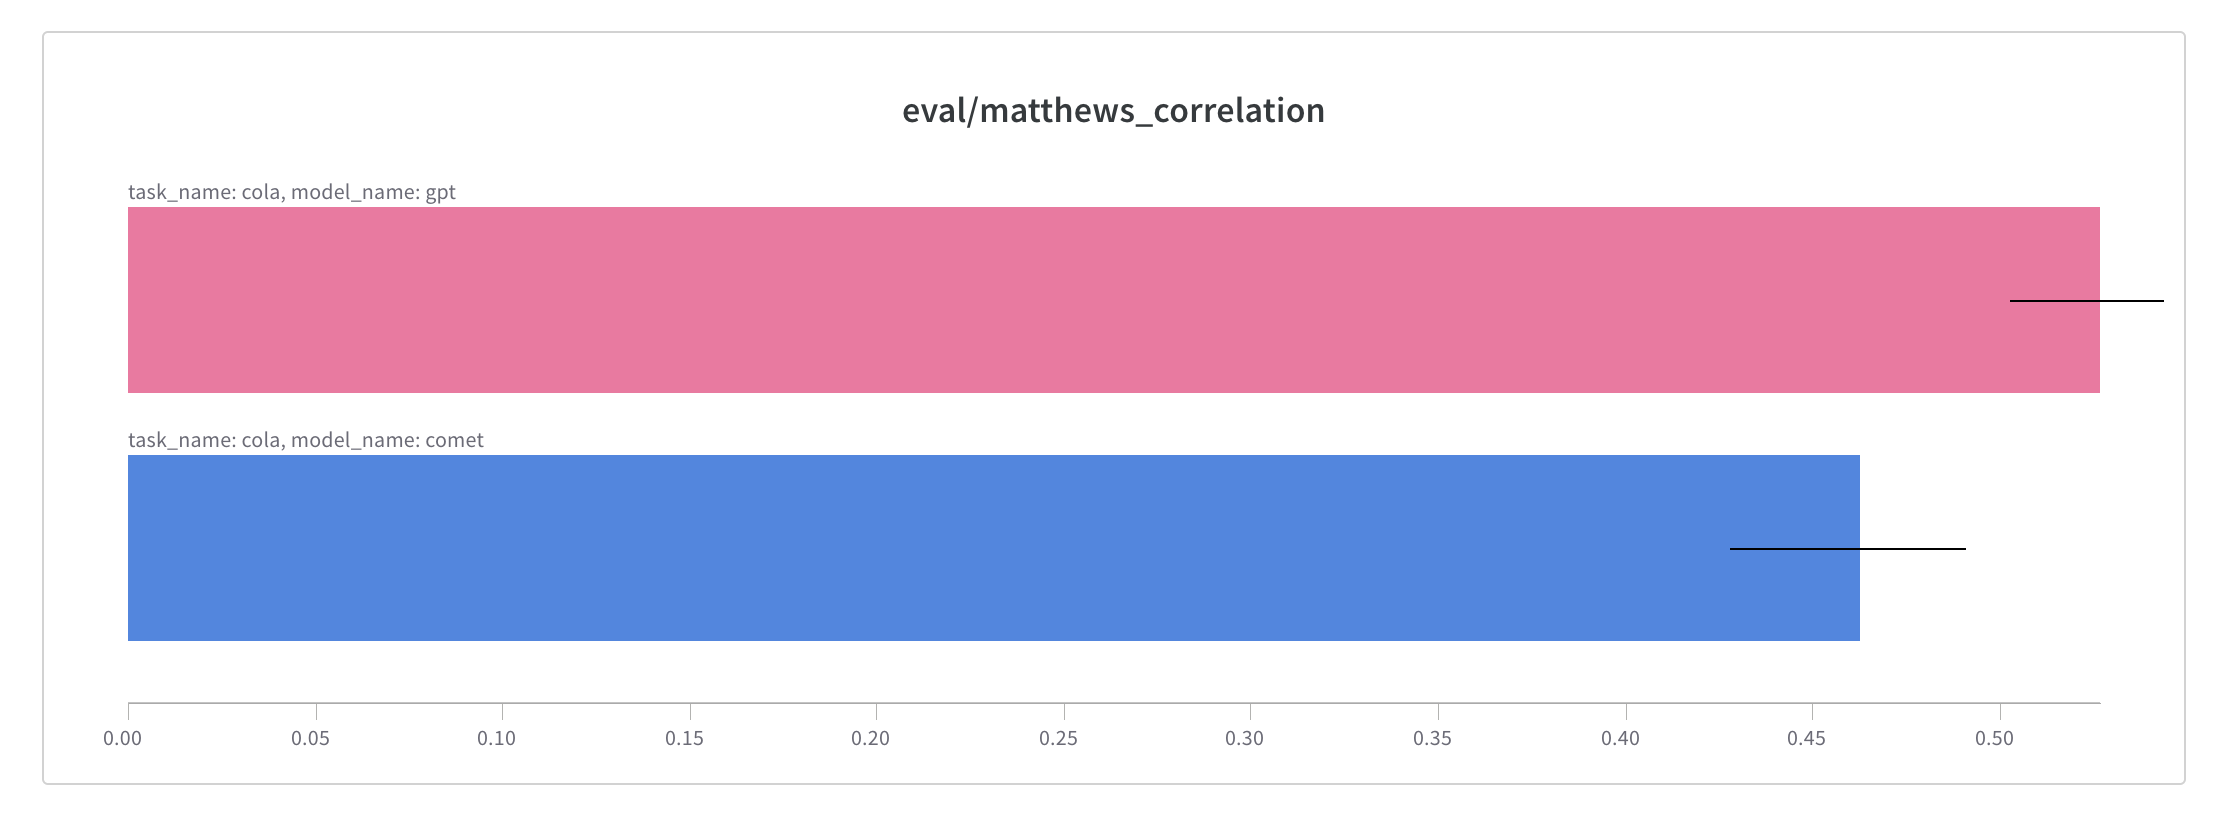
\includegraphics[keepaspectratio=true, width=0.9\textwidth]{\main/img/COLA}
    \caption[GLUE Results: CoLA] {GLUE Results: CoLA}
    \label{fig:cola_fig}
    % Put the label *after* the caption, but inside the float
\end{figure}


In order to understand how our models differ, we analyzed the results from the COLA task further. 
We used the validation subset and made predictions on it. Then we compared the predictions between
the two models and the ground truth. We saw that there were 160 instances from the total 
subset of 1043 instances where the two models disagreed. 

The Corpus of Linguistic Acceptability (CoLA) task is focused on a model's ability 
to recognize a malformed sentence (gramatically). An example of a malformed sentence that is 
part of the dataset is `Who does John visit Sally because he likes'. 

Upon Analyzing our results for the CoLA task, we noticed that the COMET 
model struggled with instances where something was happening in the past tense.

An example of this would be `There presented itself a wonderful opportunity yesterday.' 
This is supposed to be a malformed sentence. The un-specialized GPT2-xl model is able to 
recognize it as such but the COMET model fails to do so. 

\section{RTE Results}\label{sec:rte_results}


\end{document}